\documentclass{llncs}
\usepackage{amssymb}
\usepackage{graphicx}
\usepackage[ruled,linesnumbered,boxed]{algorithm2e}
\usepackage{graphicx}
\usepackage{amsmath}
%\usepackage{mathtools}
%\usepackage{color}
\usepackage{tabularx}
\usepackage[colorlinks, linkcolor=blue, anchorcolor=blue, citecolor=green]{hyperref}
%\usepackage{booktabs}
\usepackage[table]{xcolor}
%\uespackage{colortbl}
\usepackage[tight,footnotesize]{subfigure}
\usepackage{fancyhdr}
\usepackage{lastpage}
\usepackage{layout}
%\usepackage{ctex}

%\footskip = 10pt
\pagestyle{fancy}
\chead{Group Project}
\lhead{CS214-Algorithm@SJTU}
\rhead{Instructor: Xiaofeng Gao}
\rfoot{}
\cfoot{Page \thepage \ of \pageref{LastPage}}
\addtolength{\headheight}{0.5\baselineskip}
\addtolength{\headwidth}{0\marginparsep}
\addtolength{\headwidth}{0\marginparwidth}



\title{Package Delivery on ``Double 11'' Day}
\subtitle{Project for Algorithm and Complexity \vspace{-3mm}}

\author{
Kylin Chen (517030910155, k1017856853@icloud.com) \\
Fangyu Ding (517030910235, arthur\_99@sjtu.edu.cn) \\
Hongzhou Liu (517030910214, deanlhz@sjtu.edu.cn)
  }

\institute{Department of Computer Science, \\ Shanghai Jiao Tong University, Shanghai, China}

\begin{document}
\bibliographystyle{splncs}

%\linespread{0.85}

%==============================================================================
\maketitle
\begin{abstract}\vspace{-5mm}
Package delivery is such a significant problem nowadays. The convenience and speediness of online shopping highly rely on an efficient and well-organized delivery network.
Meanwhile, the delivery companies always want to reduce the cost of transportation while winning high rates from customers. The problem can be modelled as min-cost commodity flows over time.
The characteristics of such kind of problem are networks with capacities and transit times. We also have other properties like the priority of orders of commodities, the ordering time and transportation restrictions 
with respect to special kinds of commodities. However, such kind of problems is really hard to solve. Though static $s$-$t$ flow problem can be solved in polynomial time, the problem we encountered is almost NP-Hard with enormous input size.
Thus, we came up with some approximations to get good feasible solutions, applied these algorithms in different scenes and compared their performance.

\textbf{Keywords:} Package Delivery, Network Flow, Routing, Flow over time.
\end{abstract}

\setcounter{section}{-1}
\section{Symbol Table}
Define all the symbols that will be used later.
\begin{table}
\caption{Symbol Table}\label{sym1}
\centering
\begin{tabular}{|l|l|}
\hline
Symbol &  Attribute \\
\hline
$city$ & $index$, $kind(large/small/hub)$, $capacity$\\
\hline
$tool$ & $departure\_city$, $arrival\_city$, $time$, $average\_delay$, $departure\_time$, $unit\_cost$, $type$ \\
\hline
$commodity$ & $index$, $unit\_weight$, $type$ \\
\hline
$order$ & $seller\_city$, $purchaser\_city$, $order\_time$, $commodity\_index$, $amount$, $emergency$ \\
\hline
\end{tabular}
\end{table}

\section{Problem 1}
\subsection{Problem Analysis}
In this part SF Express has its substations on all 656 cities covered in the orders. We came up with a network model. Regard $city$ as vertex and $tool$ as edge, 
we can construct a network and simulate the transportation of orders on it. Our cost function is defined as $$C(p)=transport\_time^{rate}  \times transport\_cost$$
Here $p$ is the path that a particular order takes. And we evaluate the path using our cost function by the time the order takes from the time it was made to the time the 
package was sent to the consumer. We add an exponential $rate$ to represent the weight of time in the cost function. \\
The problem is an $NPO$ problem, we give the formal definition as follows:
\begin{itemize}
  \item $I$: The network model $G=(V,E)$ and the set of $order$
  \item $sol$: A set of paths $P$ representing the delivery scheme
  \item $m$: $m(G,order)=\sum_{p \in P}C(p)$
  \item $goal$: $min$
\end{itemize}
We consider that the problem is not a $LP$ or $ILP$ problem. Because the $transport\_time$ here is not linear. For example, there exist some orders that cannot be sent in the same day it was ordered. 
They will be delayed for several days thus the $transport\_time$ of a certain order will be a piecewise function.
So we defined a non-linear object function, and constructed such network model.
\subsection{Algorithm Design}
\begin{algorithm}
  \KwIn{$G$, $source\_city$, $target\_city$, $order\_time$, $arrival\_time$
        , $visited[]$, $path$, $MIN$, $optimal\_path$, $depth\_limit$}
  \BlankLine
  \caption{$dfs$}
  \label{Alg-dfs-with-depth-limit}
  
  \If{$source\_city == target\_city$ and $path$'s value $< min$ }{
    $MIN=$ $path$'s value\;
    $optimal\_path = path$\;
    $return$\; 
  }
  \If{$depth\_limit ==0$}{
    $return$\;
  }
  \BlankLine 
  
  $visited[source\_city] = true$\;
  \For{each $(city, out\_way)$ adjacent to $source\_city$}{
    \If{$visited[city]==true$ 
        and $out\_way.departure\_time \ge arrival\_time$}{
          $visited[city] = true$\;
          $path.push\_back(out\_way)$\;
          \BlankLine
          // branch-cutting-off\;
          \If{$path$'s value $< min$}{
            $dfs(G, city, target\_city, order\_time, out\_way.arrival\_time
            , visited, path, min, optimal\_path, depth\_limit - 1)$\;
          }
          \BlankLine
          $path.pop\_back()$\;
          $visited[city] = false$\;
        }
  }

\end{algorithm}
\subsection{Theoretical Analysis}
\subsubsection{Complexity Analysis}
We implemented a depth-limited DFS algorithm which technically called \textbf{iterative deepening depth-first search(IDDFS)} to search for optimal solutions. 
The time complexity is $O(b^d)$, where $b$ is the branching factor and $d$ is the depth limit.
With a depth limit, the nodes at depth $d$ are expanded once, the nodes at depth $d-1$ are expanded twice. So the total number of expansions in an IDDFS is
$$b^d + 2b^{d-1} + 3b^{d-2} + ... + (d-1)b^2 + db + (d+1) = \Sigma_{i=0}^{d} (d + 1 - i)b^i$$
where $b^d$ is the number of expansions at depth $d$, $2b^{d-1}$ is the number of expansions at depth $d-1$, and so on. Factoring out $b^d$ gives
$$b^d(1 + 2b^{-1} + 3 b^{-2} + ... + (d + 1)^{-d})$$
Now let $x = \frac{1}{b}$, then we have 
$$b^d(1 + 2x + 3x^2 + ... )$$ which converge to 
$$b^d(1 - x)^{-2}$$ for $abs(x) < 1$
Since $(1-x)^{-2}$ is a constant independent of $d$(the depth), if $b > 1$ (i.e., if the branching factor is greater than 1)\\
The time complexity is $O(b^d)$.
Besides, as we also use the strategy of \textbf{branch-cutting-off}, when the total value of the current path IDDFS has found is larger than the current optimal, IDDFS would not carry on searching more cities at this branch.\\
Therefore, the branching factor $b$ would be divided by $2$ because every time we want to carry on searching at one city, half of the out ways would be strictly \textbf{impossible to be optimal} in expectation. As a result, the factor $b$ would be divided by $2$ to be $O((\frac{b}{2})^d)$, which will significantly reduce  the time complexity. 
\subsubsection{Efficiency Analysis}
The problem is an NP problem. We can find such a certifier that given a delivery scheme we can verify the correctness order-by-order. The procedure will take polynomial time and thus the problem is NP.
\subsection{Performance Evaluation}
Problem 1 is a foundation of our project, thus we take a detailed evaluation in this part. \par
First, we will take a look at the time of transfer for the optimal path of each order. Notice that $depth=\#transfer\_time+1$
\begin{figure}[htbp]
  \centering
  \subfigure[max depth = 3]{
  \begin{minipage}[t]{0.3\linewidth}
  \centering
  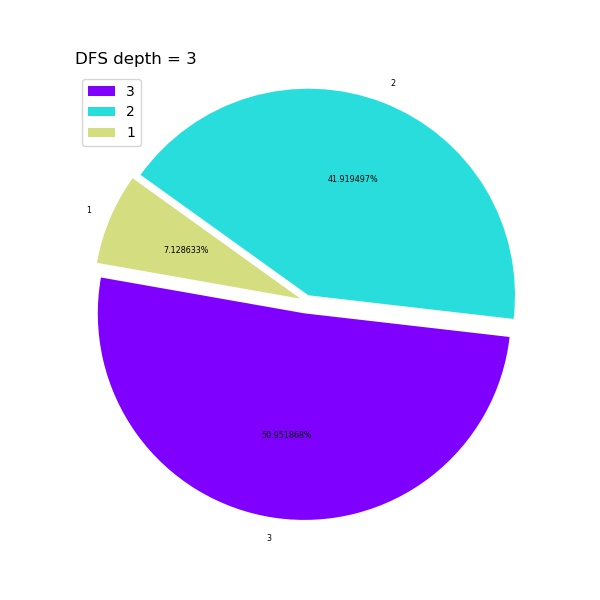
\includegraphics[width=5.5cm]{graph/Demo_official_dfs3.jpg}
  \end{minipage}
  }
  \subfigure[max depth = 4]{
  \begin{minipage}[t]{0.3\linewidth}
  \centering
  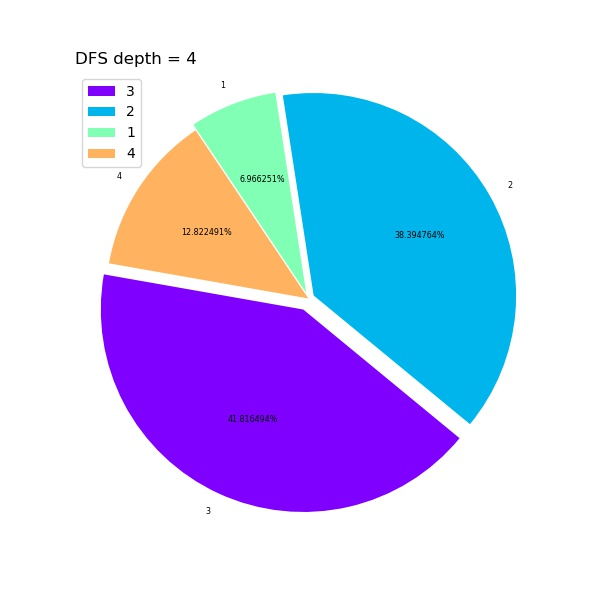
\includegraphics[width=5.5cm]{graph/Demo_official_dfs4.jpg}
  \end{minipage}
  }
  \subfigure[max depth = 6]{
  \begin{minipage}[t]{0.3\linewidth}
  \centering
  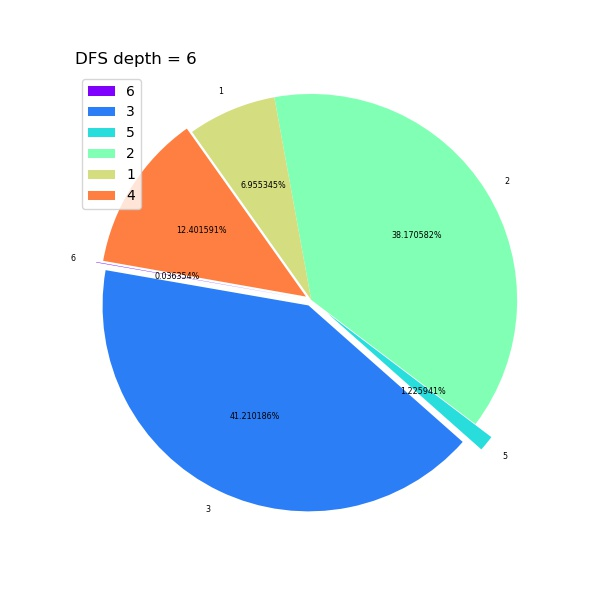
\includegraphics[width=5.5cm]{graph/Demo_official_dfs6.jpg}
  \end{minipage}
  }
  \centering
  \caption{DFS depth}
\end{figure}
In our algorithm, we set a limitation of search depth. Once a certain order can find its optimal path under this limitation, we are sure it's an optimal solution. If not, we will let those 
orders who will not find it's optimal under the limitation, we will make it wait in some city and find a suboptimal solution.
As we can see in these three graphs, with the increasing of limitation of depth, some part our pie chart decreased, which means some suboptimal solutions become optimal ones due to the increasing 
of the searching limitation. But increasing the limitation will bring us heavily computation cost and the worst circumstance will have limitation of 656, which is unaffordable to find all optimal solutions.
However, we found that the proportion of orders which will take longer path to find their optimal is relatively small, thus we can take smaller depth limitation to make it an approximate algorithm. In the Problem 1-3, we choose the limitation as 4.\par

Second, we will discuss the choice of parameter $rate$ in our object function $C(p)$. We ran some testing programs and drew a graph to show the effect of our cost function on the decision of choosing paths in our algorithm.
As we can see as long as the increasing of $rate$ the weight of time cost decreased sharply. It means that it will be hard to evaluate the cost if we choose a relatively large $rate$ for it will hide the contribution of time cost.
So we choose $rate=\dfrac{1}{2}$ in our project to make a fair cost function to evaluate the performance.

In the third part, we analyze the approximation ratio. Notice that in our project we choose the depth of IDDFS as 4. So our approximate algorithm is IDDFS with depth of 4.
However, it's really hard to compute the approximation ratio mathematically. We would rather compute the approximation ratio by comparing the result of our algorithm. As we 
mentioned before, the algorithm will surely find the global optimal if we set the depth as 656. It's because there're no negative loops in our network model and the depth of 656 implies that we will search all the 
possible paths. 
\begin{figure}[htbp]
  \centering
  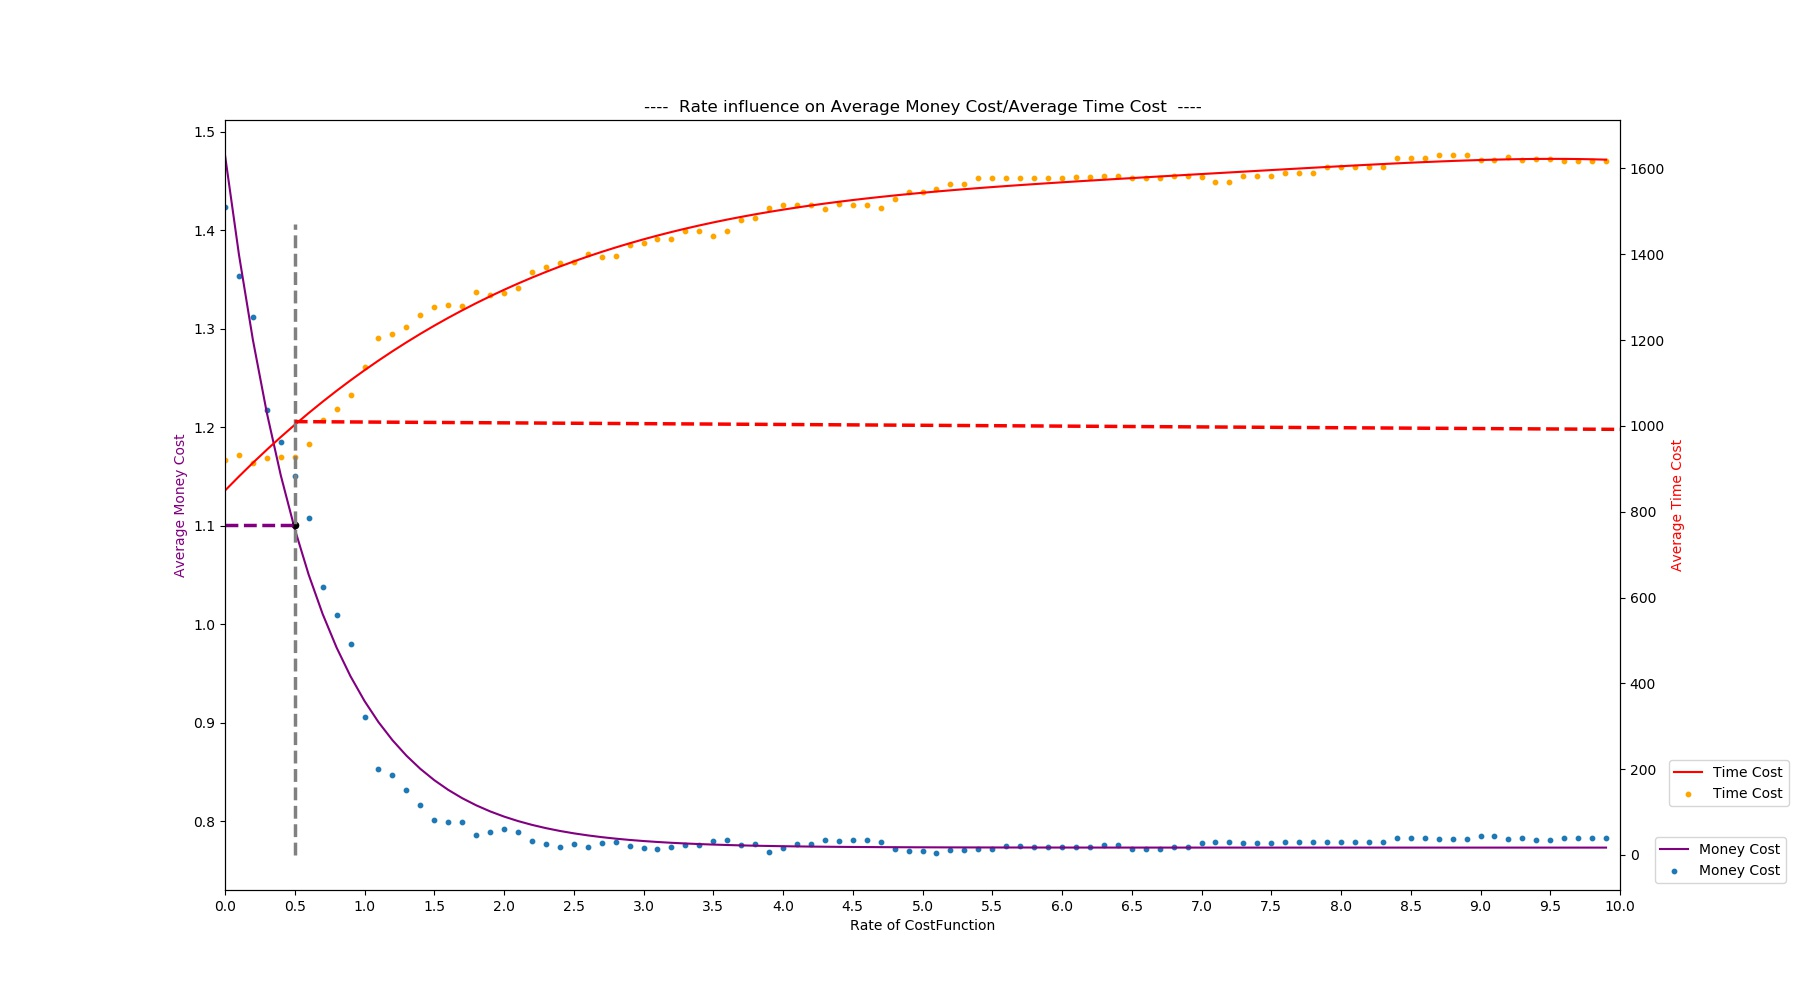
\includegraphics[height = 7cm]{graph/Rate.jpg}
  \caption{Rate}
  \label{fig:rt}
\end{figure}
\section{Problem 2}
\subsection{Problem Analysis}
In this section, we set some hubs in some cities. Hubs can gather packages and send them together to the same city with lower unit cost. However, the packages gathered together at a hub to one
destination can only be sent by one transportation tool. We defined some new symbols \\
\begin{table}
  \caption{Problem 2 Symbols}\label{sym2}
  \centering
  \begin{tabular}{|l|l|}
  \hline
  Symbol &  Definition \\
  \hline
  $\hat{C}$ & The cost of setting a hub, a constant\\
  \hline
  $discount$ & The discount rate on the cost when packages are sent from the same hub, $discount\in (0,1)$\\
  \hline
  $\#hub$ & The number of hubs \\
  \hline
  $H$ & The set of cities where hubs are set \\
  \hline
  \end{tabular}
\end{table}
We consider it's an $NPO$ problem as well.
\begin{itemize}
  \item $I$: The network model $G=(V,E)$, the set of $order$, the set of hubs $H$
  \item $sol$: A set of paths $P$ representing the delivery scheme
  \item $m$: $m(G,order,H,\hat{C},discount)=\sum_{p \in P}C(p)$.
  \item $goal$: $min$
\end{itemize}
\subsection{Algorithm Design}
First, we designed the algorithm to choose suitable cities to set hubs.
Then, we designed the algorithm to find a new delivery scheme.
\begin{algorithm}
  \KwIn{$G$, $out\_ways\_of\_hub$, $source\_city$, $target\_city$, $order\_time$, $arrival\_time$
        , $visited[]$, $path$, $MIN$, $optimal\_path$, $depth\_limit$}
  \BlankLine
  \caption{dfs with hubs}
  \label{Alg-dfs-with-hubs}
  
  \If{$source\_city == target\_city$ and $path$'s value $< min$ }{
    $MIN=$ $path$'s value\;
    $optimal\_path = path$\;
    $return$\; 
  }
  \If{$depth\_limit ==0$}{
    $return$\;
  }
  \BlankLine 
  
  $visited[source\_city] = true$\;
  \If{$source\_city$ is hub}{
    \For{each $(city, out\_way)$ adjacent
         to $source\_city$ in Graph $out\_ways\_of\_hub$}{
      \If{$visited[city]==true$ 
          and $out\_way.departure\_time \ge arrival\_time$}{
            $visited[city] = true$\;
            $path.push\_back(out\_way)$\;
            \BlankLine
            \If{$path$'s value $< min$}{
              $dfs(G,out\_ways\_of\_hub , city, target\_city, order\_time, out\_way.arrival\_time
              , visited, path, min, optimal\_path, depth\_limit - 1)$\;
            }
            \BlankLine
            $path.pop\_back()$\;
            $visited[city] = false$\;
          }
    }
  }
  \Else{
    \For{each $(city, out\_way)$ adjacent to $source\_city$ in Graph G}{
      \If{$visited[city]==true$ 
          and $out\_way.departure\_time \ge arrival\_time$}{
            $visited[city] = true$\;
            $path.push\_back(out\_way)$\;
            \BlankLine
            \If{$path$'s value $< min$}{
              $dfs(G, city, target\_city, order\_time, out\_way.arrival\_time
              , visited, path, min, optimal\_path, depth\_limit - 1)$\;
            }
            \BlankLine
            $path.pop\_back()$\;
            $visited[city] = false$\;
          }
    }
  }

\end{algorithm}
\subsection{Theoretical Analysis}
\subsubsection{Complexity Analysis}

\subsubsection{Efficiency Analysis}
\subsection{Performance Evaluation}

\section{Problem 3}
\subsection{Problem Analysis}
In real case, some other constraints should be considered: the hubs may be capacitated; some hubs may not accept some specific packages; some packages
may not be transferred by some transportation tools. We listed our constraints for transportations as follows \par
\begin{table}
  \caption{Constraints on Transportations}\label{cts1}
  \centering
  \begin{tabular}{|l|l|}
  \hline
  Tool &  Constraint \\
  \hline
  Trunk & None\\
  \hline
  Train & None\\
  \hline
  Plane & Inflammable Products, Liquid \\
  \hline
  Ship & Food \\
  \hline
  \end{tabular}
\end{table}
As for constraints on hubs, we randomly set some constraints on hubs. Here, the problem is still an $NPO$, we just add some new constraints to it.
And we still cannot convert it to $LP$ or $ILP$.
\subsection{Algorithm Design}
\begin{algorithm}
  \KwIn{$G$, $source\_city$, $target\_city$, $order\_time$, $arrival\_time$
        , $visited[]$, $path$, $MIN$, $optimal\_path$, $depth\_limit, commodity\_type$}
  \BlankLine
  \caption{dfs with constraints}
  \label{Alg-dfs-with-constraints}
  
  \If{$source\_city == target\_city$ and $path$'s value $< min$ }{
    $MIN=$ $path$'s value\;
    $optimal\_path = path$\;
    $return$\; 
  }
  \If{$depth\_limit ==0$}{
    $return$\;
  }
  \BlankLine 
  
  $visited[source\_city] = true$\;
  \For{each $(city, out\_way)$ adjacent to $source\_city$}{
    \If{$visited[city]==true$ 
        and $out\_way.departure\_time \ge arrival\_time$
        and $out\_way.type$ can deliver $commodity\_type$}{
          $visited[city] = true$\;
          $path.push\_back(out\_way)$\;
          \BlankLine
          \If{$path$'s value $< min$}{
            $dfs(G, city, target\_city, order\_time, out\_way.arrival\_time
            , visited, path, min, optimal\_path, depth\_limit - 1, commodity\_type)$\;
          }
          \BlankLine
          $path.pop\_back()$\;
          $visited[city] = false$\;
        }
  }

\end{algorithm}
\subsection{Theoretical Analysis}
\subsection{Performance Evaluation}

\section{Problem 4}
\subsection{Problem Analysis}
In this problem, we suppose that the SF Express does not have substations in all cities, but only in big cities. Here we suppose that the big cities are those supporting airline service. 
This means that the SF Express should first take the packages from sellers to some substations, and when delivering the packages to purchasers, some substations should receive the packages first, and then send them to the city that the purchasers are in.
\subsection{Algorithm Design}
\begin{algorithm}
  \KwIn{$G\_among\_big\_cities$, $G\_other\_routes$, $source\_city$, $target\_city$, $order\_time$, $arrival\_time$
        , $visited[]$, $path$, $MIN$, $optimal\_path$, 
        $depth\_limit\_search\_for\_big$, $depth\_limit\_among\_big$, $depth\_limit\_leave\_from\_big$}
  \BlankLine
  \caption{dfs for deliveries only happen between big cities}
  \label{Alg-dfs-for-deliveries-only-happen-between-big-cities}
  
  \If{$source\_city == target\_city$ and $path$'s value $< min$ }{
    $MIN=$ $path$'s value\;
    $optimal\_path = path$\;
    $return$\; 
  }
  \BlankLine 
  
  //has not been in big cities (in the stage of searching for big cities)\;
  \If{source\_city is not big cities}{
    //search for a big city\;
    \If{depth\_limit\_search\_for\_big $ne 0$}{
      $visited[source\_city] = true$\;
      \For{each $(city, out\_way)$ adjacent to $source\_city$ 
      in Graph $G\_other\_routes$}{
        \If{$visited[city]==true$ 
            and $out\_way.departure\_time \ge arrival\_time$}{
              $visited[city] = true$\;
              $path.push\_back(out\_way)$\;
              \BlankLine
              \If{$path$'s value $< min$}{
                dfs($G\_among\_big\_cities$, $G\_other\_routes$, $source\_city$, $target\_city$, $order\_time$, $arrival\_time$
        , $visited[]$, $path$, $MIN$, $optimal\_path$, 
        $depth\_limit\_search\_for\_big - 1$, $depth\_limit\_among\_big$, $depth\_limit\_leave\_from\_big$)\;
              }
              \BlankLine
              $path.pop\_back()$\;
              $visited[city] = false$\;
            }
      }
    }
  }
  
  \BlankLine
  // has been in big cities\;
  \Else{
    \BlankLine
    // we can go to another big city\;
    \If{depth\_limit\_among\_big $ne 0$}{
      $visited[source\_city] = true$\;
      \For{each $(city, out\_way)$ adjacent to $source\_city$ 
      in Graph $G\_among\_big\_cities$}{
        \If{$visited[city]==true$ 
            and $out\_way.departure\_time \ge arrival\_time$}{
              $visited[city] = true$\;
              $path.push\_back(out\_way)$\;
              \BlankLine
              \If{$path$'s value $< min$}{
                dfs($G\_among\_big\_cities$, $G\_other\_routes$, $source\_city$, $target\_city$, $order\_time$, $arrival\_time$
        , $visited[]$, $path$, $MIN$, $optimal\_path$, 
        $0$, $depth\_limit\_among\_big - 1$, $depth\_limit\_leave\_from\_big$)\;
              }
              \BlankLine
              $path.pop\_back()$\;
              $visited[city] = false$\;
            }
      }
    }

    \BlankLine
    // Also, we can leave from this big city to the destination\;
    \If{depth\_limit\_leave\_from\_big $ne 0$}{
      $visited[source\_city] = true$\;
      \For{each $(city, out\_way)$ adjacent to $source\_city$ 
      in Graph $G\_other\_routes$}{
        \If{$visited[city]==true$ 
            and $out\_way.departure\_time \ge arrival\_time$}{
              $visited[city] = true$\;
              $path.push\_back(out\_way)$\;
              \BlankLine
              \If{$path$'s value $< min$}{
                dfs($G\_among\_big\_cities$, $G\_other\_routes$, $source\_city$, $target\_city$, $order\_time$, $arrival\_time$
        , $visited[]$, $path$, $MIN$, $optimal\_path$, 
        $0$, $0$, $depth\_limit\_leave\_from\_big - 1$)\;
              }
              \BlankLine
              $path.pop\_back()$\;
              $visited[city] = false$\;
            }
      }
    }
  }

  $visited[source\_city] = true$\;
  \For{each $(city, out\_way)$ adjacent to $source\_city$}{
    \If{$visited[city]==true$ 
        and $out\_way.departure\_time \ge arrival\_time$}{
          $visited[city] = true$\;
          $path.push\_back(out\_way)$\;
          \BlankLine
          \If{$path$'s value $< min$}{
            $dfs(G, city, target\_city, order\_time, out\_way.arrival\_time
            , visited, path, min, optimal\_path, depth\_limit - 1)$\;
          }
          \BlankLine
          $path.pop\_back()$\;
          $visited[city] = false$\;
        }
  }

\end{algorithm}
\subsection{Theoretical Analysis}
\subsection{Performance Evaluation}

\section{First Section}
\subsection{A Subsection Sample}
Please note that the first paragraph of a section or subsection is
not indented. The first paragraph that follows a table, figure,
equation etc. does not need an indent, either.

Subsequent paragraphs, however, are indented.

\subsubsection{Sample Heading (Third Level)} Only two levels of
headings should be numbered. Lower level headings remain unnumbered;
they are formatted as run-in headings.

\paragraph{Sample Heading (Fourth Level)}
The contribution should contain no more than four levels of
headings. Table~\ref{tab1} gives a summary of all heading levels.

\begin{table}
\caption{Table captions should be placed above the
tables.}\label{tab1}
\centering
\begin{tabular}{|l|l|l|}
\hline
Heading level &  Example & Font size and style\\
\hline
Title (centered) &  {\Large\bfseries Lecture Notes} & 14 point, bold\\
1st-level heading &  {\large\bfseries 1 Introduction} & 12 point, bold\\
2nd-level heading & {\bfseries 2.1 Printing Area} & 10 point, bold\\
3rd-level heading & {\bfseries Run-in Heading in Bold.} Text follows & 10 point, bold\\
4th-level heading & {\itshape Lowest Level Heading.} Text follows & 10 point, italic\\
\hline
\end{tabular}
\end{table}

\noindent Displayed equations are centered and set on a separate
line.
\begin{equation}
x + y = z
\end{equation}
Please try to avoid rasterized images for line-art diagrams and
schemas. Whenever possible, use vector graphics instead (see
Fig.~\ref{fig1}).

\begin{figure}
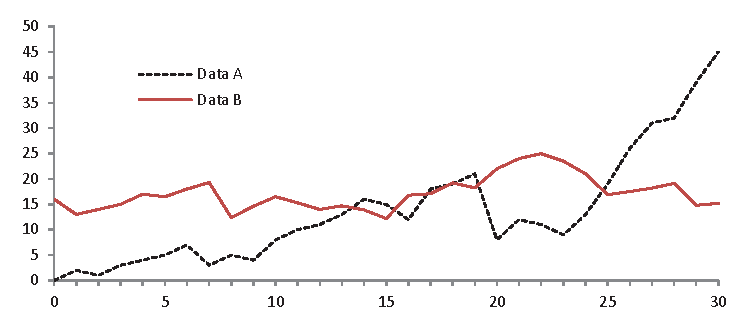
\includegraphics[width=0.6\textwidth]{fig1.eps}
\centering
\caption{A figure caption is always placed below the illustration.
Please note that short captions are centered, while long ones are
justified by the macro package automatically.} \label{fig1}
\end{figure}

\begin{theorem}
This is a sample theorem. The run-in heading is set in bold, while
the following text appears in italics. Definitions, lemmas,
propositions, and corollaries are styled the same way.
\end{theorem}
%
% the environments 'definition', 'lemma', 'proposition', 'corollary',
% 'remark', and 'example' are defined in the LLNCS documentclass as well.
%
\begin{proof}
Proofs, examples, and remarks have the initial word in italics,
while the following text appears in normal font.
\end{proof}
For citations of references, we prefer the use of square brackets
and consecutive numbers. Citations using labels or the author/year
convention are also acceptable. The following bibliography provides
a sample reference list with entries for journal
articles~\cite{ref_article1}, an LNCS chapter~\cite{ref_lncs1}, a
book~\cite{ref_book1}, proceedings without editors~\cite{ref_proc1},
and a homepage~\cite{ref_url1}. Multiple citations are grouped
\cite{ref_article1,ref_lncs1,ref_book1},
\cite{ref_article1,ref_book1,ref_proc1,ref_url1}.


\section*{Acknowledgements}

Here is your acknowledgements. You may also include your feelings, suggestion, and comments in the acknowledgement section.

%
% ---- Bibliography ----
%
% BibTeX users should specify bibliography style 'splncs04'.
% References will then be sorted and formatted in the correct style.
%
% \bibliographystyle{splncs04}
% \bibliography{mybibliography}
%
\begin{thebibliography}{8}
\bibitem{ref_article1}
Author, F.: Article title. Journal \textbf{2}(5), 99--110 (2016)

\bibitem{ref_lncs1}
Author, F., Author, S.: Title of a proceedings paper. In: Editor,
F., Editor, S. (eds.) CONFERENCE 2016, LNCS, vol. 9999, pp. 1--13.
Springer, Heidelberg (2016).

\bibitem{ref_book1}
Author, F., Author, S., Author, T.: Book title. 2nd edn. Publisher,
Location (1999)

\bibitem{ref_proc1}
Author, A.-B.: Contribution title. In: 9th International Proceedings
on Proceedings, pp. 1--2. Publisher, Location (2010)

\bibitem{ref_url1}
LNCS Homepage, \url{http://www.springer.com/lncs}. Last accessed 4
Oct 2017
\end{thebibliography}
\end{document}
